\documentclass{beamer}%[handout]
\mode<handout>{
\usepackage{pgfpages}
\pgfpagesuselayout{4 on 1}[letterpaper,border shrink=5mm, landscape]
}
\usepackage[T1]{fontenc}
\usepackage[utf8]{inputenc}
\usepackage[spanish]{babel}
\usepackage{beamerthemeshadow,beamerthemesplit,cite,cancel,lmodern,eso-pic,fancyvrb,textcomp,lmodern,url,times,booktabs,amssymb,amsmath,ragged2e,float,subfig,xspace,epic,eepic,multicol,multirow,colortbl,color,graphicx,url}
\usepackage{listings} %CODIGOs
\usepackage[utf8]{inputenc}
\usepackage[all]{xy}
\usepackage{multicol}
\setcounter{tocdepth}{3}


%Colores Ulagos
\definecolor{gray97}{gray}{.97}
\definecolor{gray75}{gray}{.75}
\definecolor{gray45}{gray}{.45}
\definecolor{listinggray}{gray}{0.9}
\definecolor{lbcolor}{rgb}{0.9,0.9,0.9}
%Colores Ulagos
\definecolor{amarillo}{RGB}{255,182,18}
\definecolor{verde}{RGB}{52,178,51}
\definecolor{rojo}{RGB}{237,41,57}
\definecolor{azulu}{RGB}{19,15,204}
\definecolor{azul}{RGB}{1,110,185}
\definecolor{negro}{RGB}{35,31,32}
\definecolor{naranjo}{RGB}{251,79,20}
\newcommand\rojo[1]{\textcolor[RGB]{237,41,57}{#1}}
\newcommand\gris[1]{\textcolor[gray]{.65}{#1}}
\newcommand\azul[1]{\textcolor[RGB]{19,15,204}{#1}}
\newcommand\verde[1]{\textcolor[RGB]{5,101,99}{#1}}
\newcommand\naranjo[1]{\textcolor[RGB]{251,79,20}{#1}}

%%%%%%%%%%%%%%%%%%%%%TEMA
\mode<presentation>
\usetheme{CambridgeUS}
\usecolortheme[named=azul]{structure}
 \usefonttheme[onlymath]{serif}
  \setbeamercovered{transparent}
  \setbeamertemplate{blocks}[rounded][shadow=true]
\setbeamercolor*{palette primary}{use=structure,fg=azul,bg=listinggray}
\setbeamercolor*{palette secondary}{use=structure,fg=azul,bg=gray97}
\setbeamercolor*{palette tertiary}{use=structure,fg=gray97,bg=azul}
\setbeamercolor*{palette sidebar primary}{use=structure,fg=azul}
\setbeamercolor*{palette sidebar tertiary}{use=structure,fg=azul}
\setbeamercolor{frametitle right}{bg=azul!50!white}
\setbeamercolor{structure}{fg=azul}
\setbeamerfont{block title}{size={}}
\setbeamertemplate{blocks}[rounded][shadow=true]
\setbeamercolor*{title}{use=structure,fg=black}
\setbeamertemplate{title page}[default][colsep=-4bp,rounded=false,shadow=false]
\setbeamercolor*{author}{use=structure,fg=black}
\setbeamercolor*{institute}{use=structure,fg=black}
\setbeamercolor{block title}{use=structure,fg=white,bg=amarillo}
\setbeamercolor{block body}{use=structure,fg=negro,bg=amarillo!20!white}
\setbeamercolor{block title example}{use=structure,fg=white,bg=verde!80!black}
\setbeamercolor{block body example}{use=structure,fg=negro,bg=verde!20!white}
\setbeamercolor{block title alerted}{use=structure,fg=white,bg=rojo!90!negro}
\setbeamercolor{block body alerted}{use=structure,fg=negro,bg=rojo!20!white}
\setbeamertemplate{frametitle continuation}
%%%%%%%%%%%%%%%%%%%%%FIN TEMA

%lstlisting %%%%%CODIGOS
\lstset{tabsize=4,language=C,basicstyle=\small,upquote=true,aboveskip={1.1\baselineskip},columns=fixed,showstringspaces=false, extendedchars=true,breaklines=true, prebreak = \raisebox{0ex}[0ex][0ex]{\color{gray75}{\ensuremath{\hookleftarrow}}},showtabs=false,showspaces=false,showstringspaces=false,identifierstyle=\ttfamily,keywordstyle=\color[rgb]{0,0,1}, commentstyle=\color[rgb]{0.133,0.545,0.133}, stringstyle=\color[rgb]{0.627,0.126,0.941}} 
  
%%%%%%%%%%%%%%PORTADA
\logo{\centering
\includegraphics[height=1cm,width=1cm]{unet.jpg}}
\title[HIVmlm]{\textbf{\small{Desarrollo de una aplicaci\'on web para el estudio de los datos longitudinales para el seguimiento de la infecci\'on por el virus de inmunodeficiencia humana, caso de estudio: IAHULA}}}
\author{\textbf{Stephanie Correa}}
\institute[UNET]{}
\date[]{Julio 2018}
%%%%%%%%%%%%%FIN PORTADA

\begin{document}
\setbeamertemplate{background}{\centering
\includegraphics[height=9.2cm,width=12.8cm]{hiv.jpg}}
\setbeamertemplate{navigation symbols}{}
%%%%%%%%%%%%%%%PAGINA DE PORTADA
\begin {frame} [plain]

\vspace{3 cm}
\titlepage
\end {frame}


\setbeamertemplate{background}{}

%%%%%%%%%%%%%%%%ÍNDICES
\section[Indice]{}
\frame{
  \frametitle{\textbf{Indice}}
\setcounter{tocdepth}{5}%1: solo titulo principal, 2: titulo y subtitulo, 3....
\scriptsize
\tableofcontents[]
}%Generacion de Indice por capitulo


%%%%%%%%%%%%%%%%FIN ÍNDICES

%%%%%%%%%%%%%%%%%%%%%%%%%%%%%%%%%%%%%
%%%%%%%%%%%%%%%%%INICIO PRESENTACION

\section{El problema}

\begin{frame}[fragile]
\frametitle{\textbf{Planteamiento del problema}}
\begin{block}{Puntos clave}
\end{block}
\begin{itemize}
\item Seguimiento de la infecci\'on por VIH
\item An\'alisis temporal
\item Datos longitudinales
\end{itemize}
\begin{equation}
\notag
 \begin{array}{lll}
y_{1} & = & \{ y_{11}, y_{12}, \cdots, y_{1n_{i}} \}                 \\
&     \vdots            &     \\
y_{i=N} & = & \{ y_{N1}, y_{N2}, \cdots, y_{Nn_{i}} \}                 \\
\end{array} \label{eq1}
\end{equation}

Con $n_i$ el n\'umero de observaciones para   $i$-\'esimo individuo (N).\\
\end{frame}

\begin{frame}[fragile]
\frametitle{\textbf{Planteamiento del problema}}
\begin{block}{Caracter\'isticas de los datos longitudinales}
\end{block}
\begin{itemize}
   \item Alta heterogeneidad
   \item Correlaci\'on entre medidas 
   \item Datos faltantes
\end{itemize}
\end{frame}

\begin{frame}[fragile]
\frametitle{\textbf{Planteamiento del problema}}
\begin{block}{Caracter\'isticas de los datos longitudinales en VIH}
\end{block}
	\begin{center}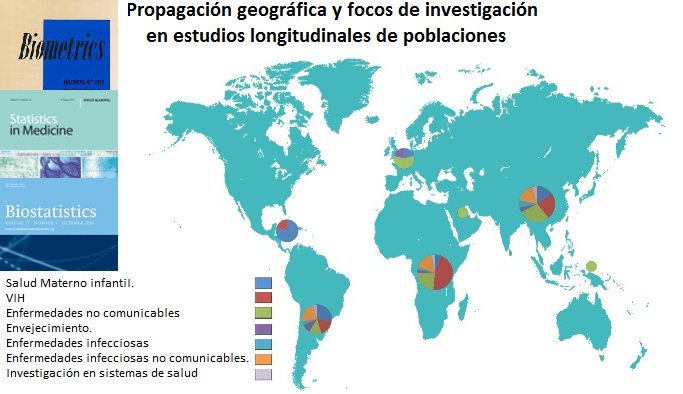
\includegraphics[height=0.5\textheight]{LON.PNG}\end{center}
\tiny{Whitworth L. Reflection on Cohorts and Longitudinal Studies. UNICEF office research. Wellcome Trust. Florence. 2014.}\\
\end{frame}
\subsection{Objetivo general}

\begin{frame}[fragile]
\frametitle{\textbf{Objetivo general}}
\begin{block}{Objetivo}
\end{block}
Desarrollar una aplicaci\'on web para el estudio de datos longitudinales para el
seguimiento\ de la infecci\'on por el Virus de  Inmunodeficiencia Humana.\\
\textcolor{blue}{Caso de estudio:} Instituto Auton\'omo Hospital Universitario de los Andes.
\end{frame}

\subsection{Objetivos espec\'ificos}
\begin{frame}[fragile]
\frametitle{\textbf{Objetivos especificos}}
\begin{block}{Objetivos}
\end{block}
\begin{itemize}
\item Diagnosticar la informaci\'on obtenida en la base de datos suministrada por el Instituto Auton\'omo Hospital Universitario de los Andes.
\item Analizar de manera exploratoria y descriptiva los datos para la selecci\'on de las variables a utilizar en el m\'odelo a implementar.
\item Implementar un m\'odelo para el manejo de datos longitudinales en una aplicaci\'on web.
\item Aplicar pruebas de funcionalidad en la aplicaci\'on.
\end{itemize}
\end{frame}

\section{Fundamentos te\'oricos}

\begin{frame}
\frametitle{\textbf{Antecedentes}}
\textbf{Manejo de datos longitudinales multivariados incompletos de alta dimensi\'on con tipos de datos mixtos por imputaci\'on m\'ultiple utilizando un m\'odelo de an\'alisis factorial longitudinal}
 \begin{columns}[t]
    \column{0.4\textwidth}
	\begin{itemize}
	\item Modelo escrito en R
	\item An\'alisis de factores y modelo lineales de efectos mixtos
	\item PAN - Imputaci\'on Multiple para Panel Multivariado
	\item MICE - Imputaci\'on Multiple usando Ecuaciones Encadenadas 
	\end{itemize}
    \column{0.4\textwidth}
  	\begin{center}
\includegraphics[height=0.3\textheight]{r.PNG}\end{center}
  \end{columns}

\end{frame}

\begin{frame}
\frametitle{\textbf{Antecedentes}}
\textbf{Tablas de modelo de vida calibradas por VIH para países con epidemias de VIH generalizadas}
 \begin{columns}[t]
    \column{0.4\textwidth}
	\begin{itemize}
	\item Paquete de R HIV.LifeTables
	\item Tasa de mortalidad
	\item Prevalencia del VIH
	\item Esperanza de vida al nacer
	\end{itemize}
    \column{0.4\textwidth}
  	\begin{center}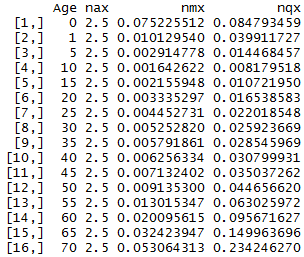
\includegraphics[height=0.4\textheight]{HIVTables.PNG}\end{center}
  \end{columns}
\end{frame}

\begin{frame}
\frametitle{\textbf{Antecedentes}}
\textbf{Uni\'on del modelado de datos longitudinales y de supervivencia}
\begin{columns}[t]
    \column{0.4\textwidth}
	\begin{itemize}
	\item Paquete de R JM
	\item Datos longitudinales
	\item Datos de supervivencia
	\item Eficacia de antirretrovirales
	\end{itemize}
    \column{0.4\textwidth}
  	\begin{center}\includegraphics[height=0.4\textheight]{JM.PNG}\end{center}
  \end{columns}

\end{frame}

\section{Metodolog\'ia}
\subsection{Poblaci\'on y muestra}

\begin{frame}
\frametitle{\textbf\textbf{Metodolog\'ia}}
\begin{block}{Poblaci\'on y muestra - Adquisici\'on y filtrado}
\end{block}
\begin{center}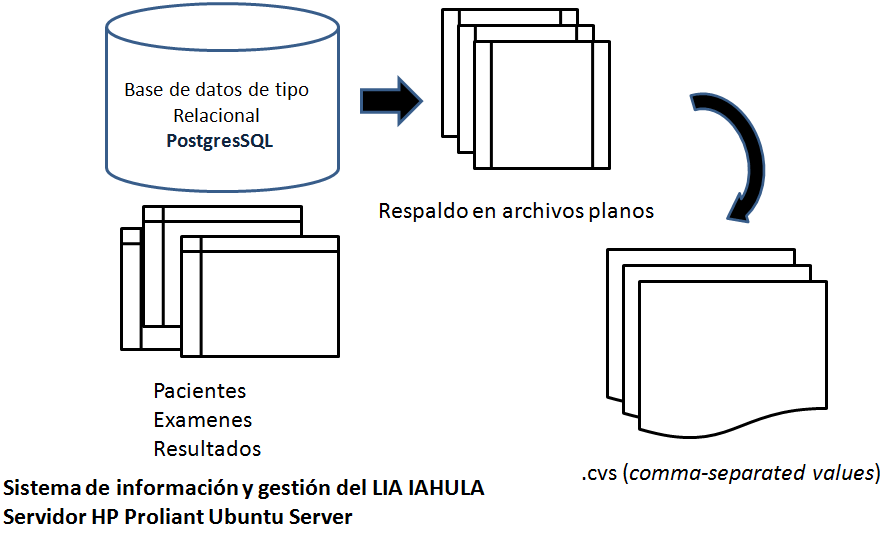
\includegraphics[height=0.5\textheight]{PM.PNG}\end{center}
\tiny{\textcolor{blue}{Poblaci\'on de pacientes registrada entre enero del a\~no 2007  hasta diciembre del a\~no 2013:  45649 pacientes.}}
\end{frame}


\begin{frame}
\frametitle{\textbf\textbf{Metodolog\'ia}}
\begin{block}{Adquisici\'on - Ejemplo de una vista minable}
\end{block}
\begin{center}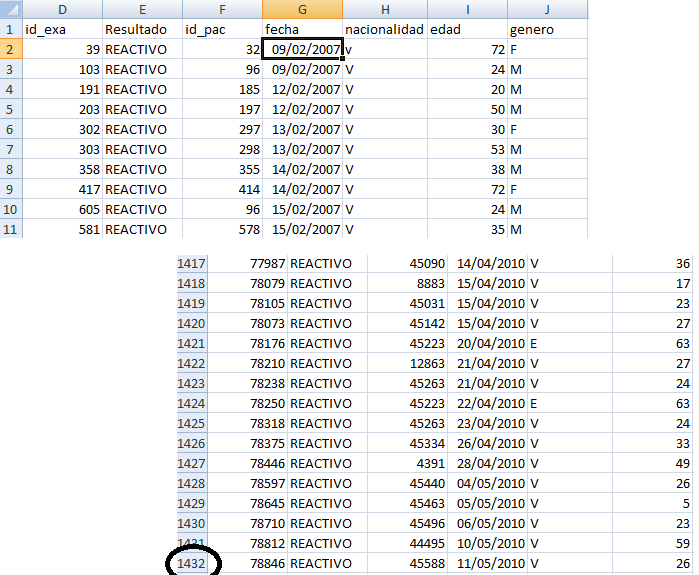
\includegraphics[height=0.5\textheight]{VM1.PNG}\end{center}

\tiny{\textcolor{blue}{Vista minable de la ventana de tiempo entre enero del a\~no 2007 y marzo del a\~no 2010 reportaba 1431 pacientes reactivos para VIH.}}

\tiny{Seg\'un el Informe nacional de seguimiento de la declaraci\'on pol\'itica sobre VIH y el SIDA de 2011.  MPPS.  ente los a\~nos 2007 y 2010 se reportaron 47.771 nuevos casos (Tabla 4. Pag. 21)}

\end{frame}


\begin{frame}
\frametitle{\textbf\textbf{Metodolog\'ia}}
\begin{block}{Filtrado de la vistas minables}
\end{block}
\small{
\begin{itemize}
    \item La base de datos del Laboratorio de Investigaciones Hormonales IAHULA, no s\'olo almacena informaci\'on del Programa de Pacientes con VIH, las vistas minables estan conformadas por pacientes confirmados por las pruebas \textit{Elisa} y \textit{Western Blot} para VIH
    \item En las vistas minables para  las pruebas s\'olo se categorizar\'an pacientes con residencia en el Estado Mérida
    \item Las vistas minables s\'olo las integraran pacientes con m\'as de tres años en seguimiento. Dado que los modelos son para datos longitudinales.
    \item Se categorizaron los pacientes por semestres y en cada lapso en medicados y no medicados.
\end{itemize}
}
\end{frame}

\begin{frame}
\frametitle{\textbf\textbf{Metodolog\'ia}}
\begin{block}{Filtrado de la vistas minables}
\end{block}
\begin{center}
\includegraphics[height=0.1\textheight]{MU.jpg}\end{center}
\small{Archivo para las pruebas funcionales.}
	
\tiny{
\begin{itemize}
 \item 115 registros de pacientes (Todos medicados con antiguedad $<$ 6 meses) mayores a 18 a\~nos.
 \item Secci\'on transversal: edad el g\'enero y el municipio de residencia  
 \item Secci\'on longitudinal ( Enero del año 2007 - Diciembre del año 2013)l Log$_{10}$ de la carga viral plasm\'atica y las sub-poblaciones linfocitaria de c\'elulas T$^{+}$ CD4 y  T$^{+}$ CD8.
\end{itemize}
}
\tiny{Seg\'un estad\'isticas del Programa para pacientes con VIH del IAHULA, en el año 2007 exist\'ian 615 pacientes adscritos al programa.} 
\end{frame}


\subsection{Metodolog\'ia de desarrollo de \textit{software} en espiral}
\begin{frame}
\frametitle{\textbf{Metodolog\'ia de desarrollo de \textit{software} en espiral}}
\begin{columns}[t]
    \column{0.4\textwidth}
  \begin{block}{Caracter\'isticas del desarrollo de \textit{software}}
  \textcolor{red}{Ciclo de vida de \textit{software}} \\
  \begin{enumerate}
  \item Determinar objetivos
  \item An\'alisis de riesgos
  \item Desarrollar, verificar y validar
  \item Planificar
  \end{enumerate}
\end{block}
  \column{0.4\textwidth}
\begin{center}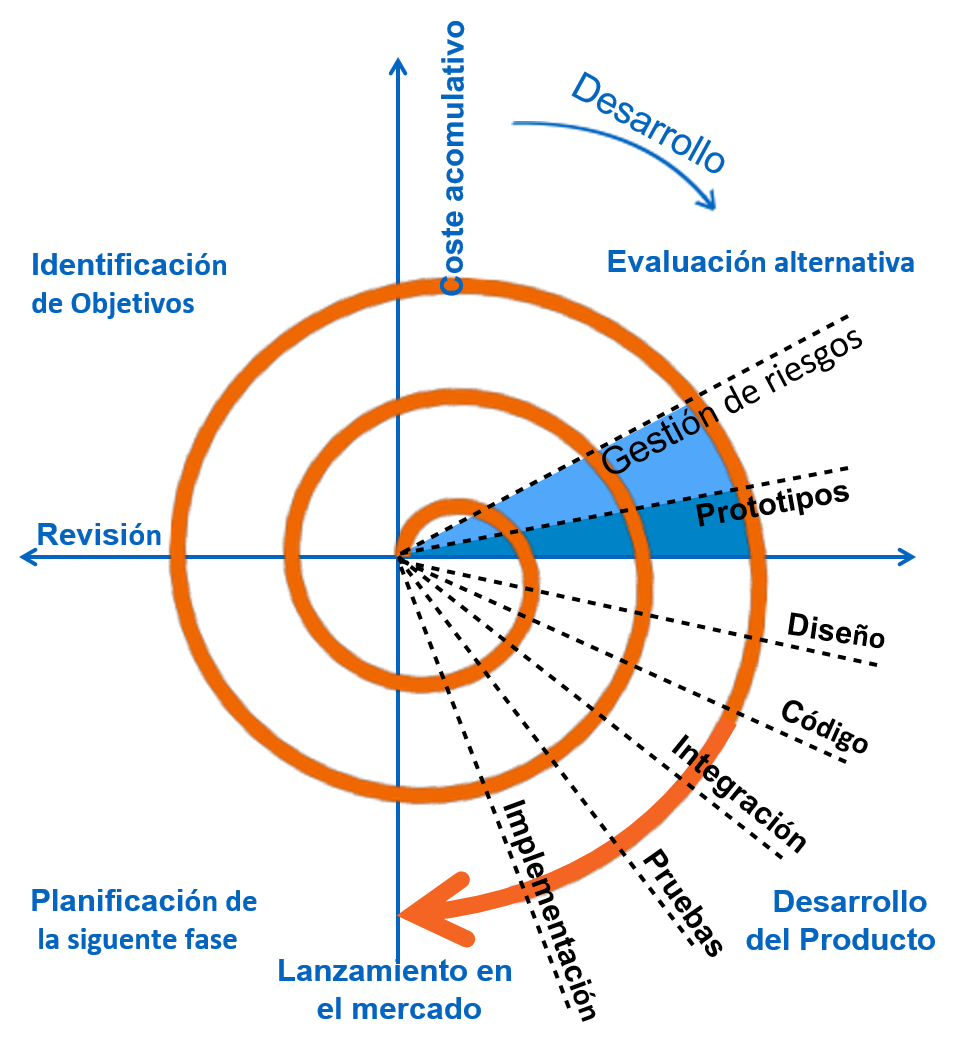
\includegraphics[height=0.6\textheight]{espiral.jpg}\end{center}
  \end{columns}
\end{frame}

\subsection{Primera interacci\'on}
\begin{frame}
\frametitle{\textbf{Prototipo 1}}
\begin{columns}[t]
    \column{0.4\textwidth}
 \begin{block}{ Primera interacci\'on}
  \begin{itemize}
  	\item Base de datos del LIA IAHULA
  	\item Implementaci\'on en lenguaje R 
  	\item Desarrollo WEB en Java
  	\item Conexi\'on R- Java con rJava y JDK eclipse.
           \item Servidor WEB (Ubuntu server)
  \end{itemize}
  	\end{block}
    \column{0.4\textwidth}
    \begin{center}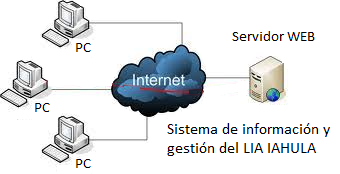
\includegraphics[height=0.3\textheight]{wireframe0.png}\end{center}
  \end{columns}
\end{frame}

\subsection{Segunda interacci\'on}

\begin{frame}
\frametitle{\textbf{Prototipo 2}}
\begin{columns}[t]
    \column{0.4\textwidth}
 \begin{block}{ Segunda interacci\'on}
  \begin{itemize}
  	\item RStudio
  	\item R
  	\item Shiny
  \end{itemize}
  	\end{block}
    \column{0.4\textwidth}
    \begin{center}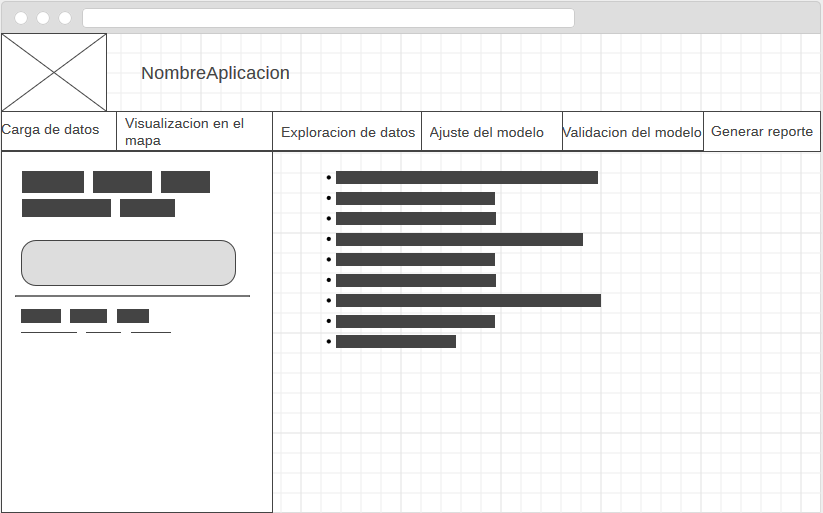
\includegraphics[height=0.4\textheight]{wireframe.png}\end{center}
  \end{columns}
\end{frame}

\section{Desarrollo - Versi\'on final HIVmlm}

\begin{frame}
\frametitle{\textbf{HIVmlm Human Immunology Virus linear model mixed effects}}
\begin{columns}[t]
    \column{0.4\textwidth}
 \begin{block}{Etapa 1}
  	HIVmlm \\
  	Creaci\'on del paquete en R \\
  	formatR\\
\end{block}
    \column{0.4\textwidth}
    M\'odulos:
    \begin{enumerate}
  	\item Carga de datos
  	\item Exploraci\'on de los datos
  	\item Visualizaci\'on en el mapa
  	\item Ajuste del modelo
  	\item Validaci\'on del modelo
  	\item Generar reporte
  \end{enumerate}
  \end{columns}
\end{frame}

\begin{frame}
\frametitle{\textbf{HIVmlm Human Immunology Virus linear model mixed effects}}
\textbf{Modelo mixto implementado}

\begin{equation}
\notag \underbrace{\textcolor{blue}{y}}_{\mbox{ Variable respuesta}} = \underbrace{\textcolor{red}{X}\beta}_{\mbox{ Efectos fijos}} + \underbrace{\textcolor{green}{Z}b}_{\mbox{ Efectos aleatorios}}+ \epsilon
\end{equation}

\small{
Donde:\\
\textcolor{blue}{La variable respuesta:}  Log$_{10}$CVP - Conteo de c\'elulas T CD4\\
\textcolor{red}{Efectos fijos:}  edad, g\'enero, lugar de residencia, grupo de riesgo, co-infecciones, (Conteo de c\'elulas T CD4  -  Log$_{10}$CVP),  Conteo de c\'elulas T CD8, entre otros.\\
\textcolor{green}{Efectos aleatorios:}  Se considera que el comportamiento de cada paciente es igual o diferente.\\
$\epsilon$ - error.}
\end{frame}

\begin{frame}
\frametitle{\textbf{HIVmlm Human Immunology Virus linear model mixed effects}}
\begin{columns}[t]
    \column{0.4\textwidth}
 \begin{block}{Etapa 2}
  	\begin{itemize}
  	\item Creaci\'on del paquete
  	\item GitHub
  	\item global.R
  	\item ui.R
  	\item server.R
  	\item reporte.Rmd
  	\end{itemize}
  	\end{block}
    \column{0.5\textwidth}
    Estructura del paquete y proyecto
    \begin{center}
\includegraphics[height=0.4\textheight]{estructura.PNG}\end{center}
  \end{columns}
\end{frame}

\begin{frame}
\frametitle{\textbf{HIVmlm Human Immunology Virus linear model mixed effects}}
\begin{columns}[t]
    \column{0.4\textwidth}
 \begin{block}{Etapa 3}
  	\begin{itemize}
  	\item IAHULA
  	\item Per\'iodo 2007 - 2013
  	\item 1610 datos registrados
  	\item 115 pacientes
  	\item Gr\'afico de torta
  	\item Histograma
  	\item Marcadores fisiol\'ogicos
  	\end{itemize}
  	\end{block}
    \column{0.5\textwidth}
    Plan de integraci\'on y pruebas
    \begin{center}
\includegraphics[height=0.4\textheight]{testthat.png}\end{center}
  \end{columns}
\end{frame}

\begin{frame}
\frametitle{\textbf{HIVmlm Human Immunology Virus linear model mixed effects}}
 
  	Carga de Archivos
  	 \begin{center}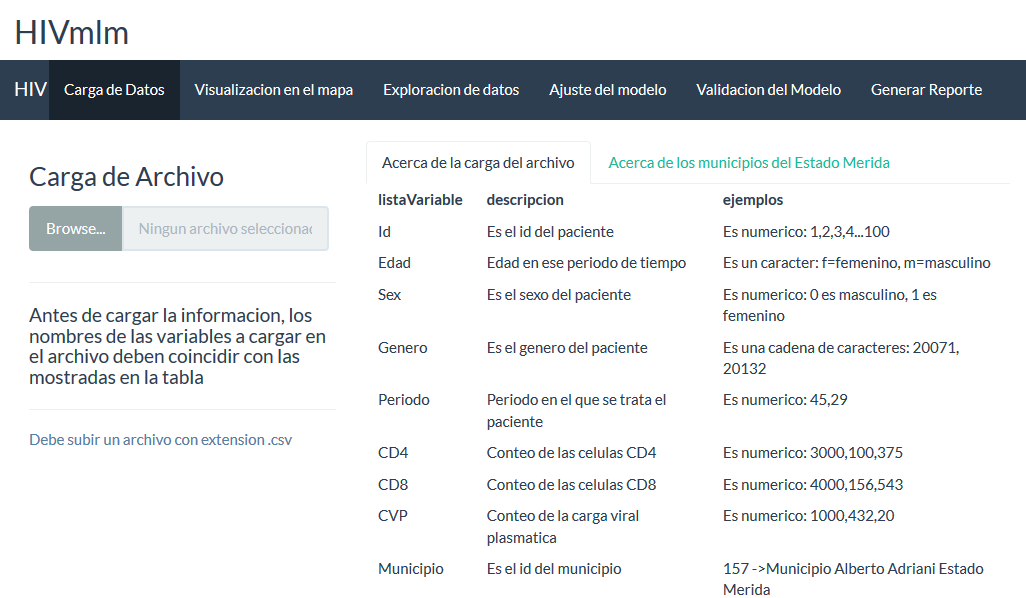
\includegraphics[height=0.6\textheight]{HIVmlm.PNG}\end{center}
  
\end{frame}

\begin{frame}
\frametitle{\textbf{HIVmlm Human Immunology Virus linear model mixed effects}}
 
  	Visualizaci\'on en el mapa
  	 \begin{center}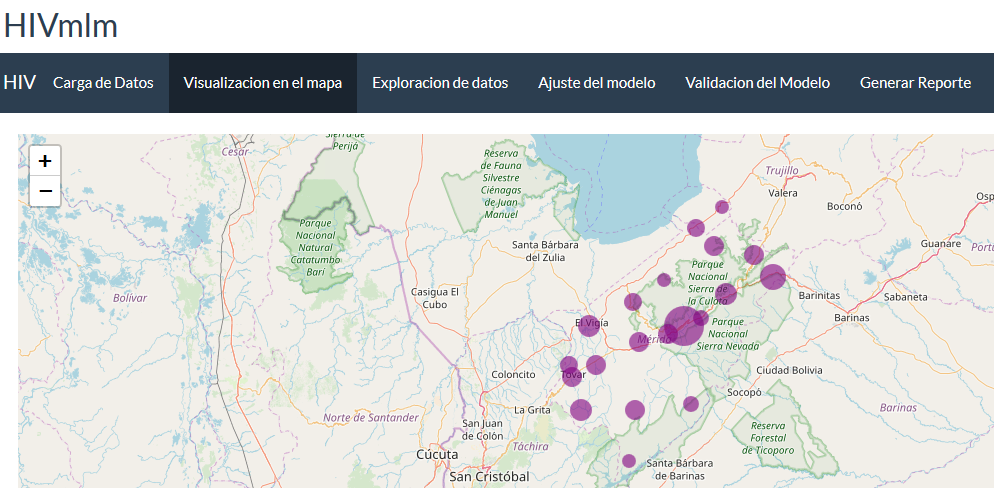
\includegraphics[height=0.6\textheight]{mapa.PNG}\end{center}
  
\end{frame}

\begin{frame}
\frametitle{\textbf{HIVmlm Human Immunology Virus linear model mixed effects}}
 
  	Exploraci\'on de los datos
  	\begin{columns}[t]
    \column{0.4\textwidth}
 \begin{center}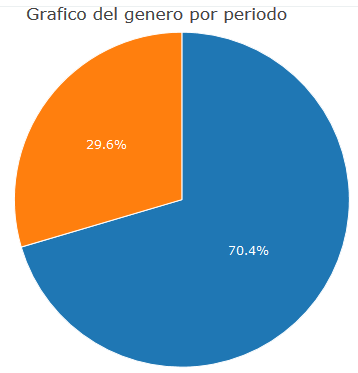
\includegraphics[height=0.3\textheight]{torta.PNG}\end{center}
    \column{0.5\textwidth}
   
    \begin{center}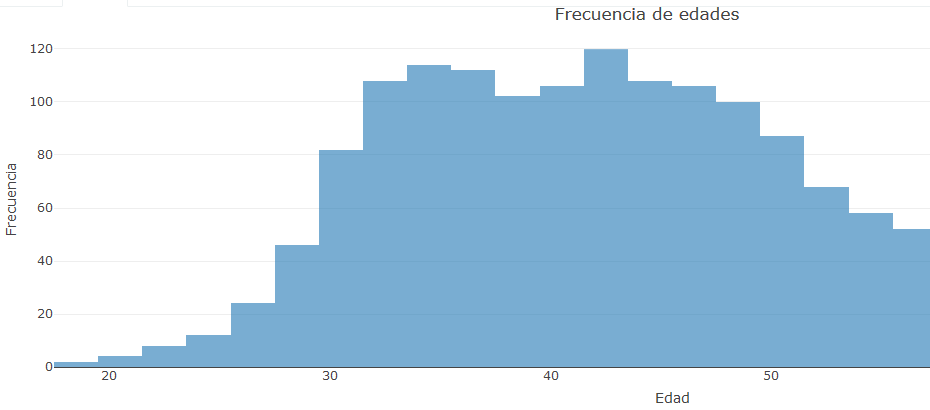
\includegraphics[height=0.3\textheight]{histograma.PNG}\end{center}
  \end{columns}
 
\end{frame}

\begin{frame}
\frametitle{\textbf{HIVmlm Human Immunology Virus linear model mixed effects}}
 
  	Ajuste del modelo
  	 \begin{center}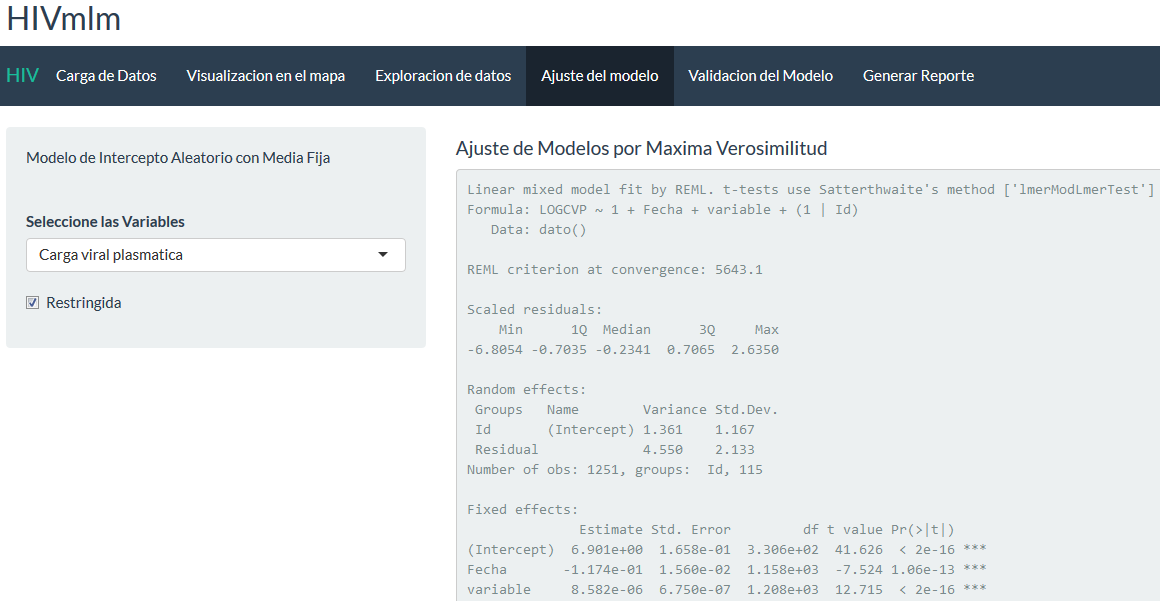
\includegraphics[height=0.6\textheight]{ajuste.PNG}\end{center}
  
\end{frame}

\section{Conclusiones y recomendaciones}


\begin{frame}
\frametitle{\textbf{Conclusiones}}
\begin{columns}[t]
    \column{0.4\textwidth}

  \begin{enumerate}
  \item Diagnosticar la informaci\'on obtenida en la base de datos 
  \item Analizar de manera exploratoria y descriptiva los datos
  \item Implementar un m\'odelo para el manejo de los datos longitudinales
  \end{enumerate}

    \column{0.6\textwidth}
   \begin{center}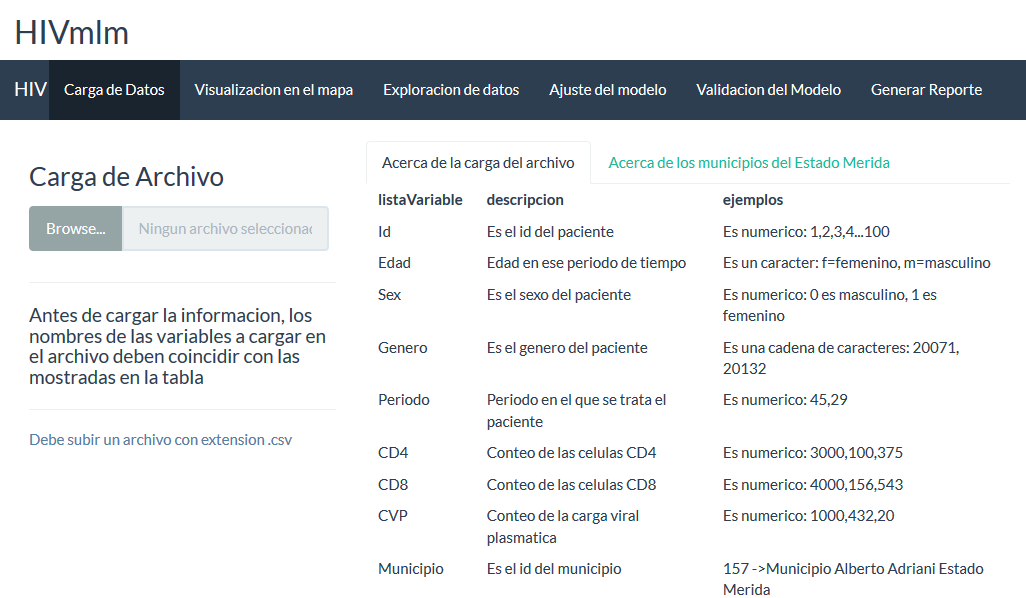
\includegraphics[height=0.4\textheight]{HIVmlm.PNG}\end{center}
  \end{columns}
\end{frame}

\begin{frame}
\frametitle{\textbf{Recomendaciones}}
\begin{columns}[t]
    \column{0.5\textwidth}
	Implementar el m\'odelo a los diferentes estados del pa\'is
	\begin{center}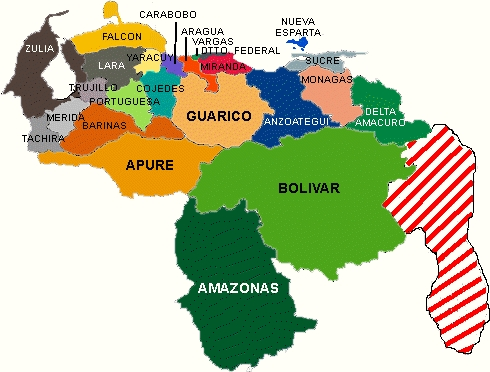
\includegraphics[height=0.4\textheight]{venezuela.jpg}\end{center}
    \column{0.5\textwidth}
    Unificar esfuerzos con organismos de salud p\'ublicos y privados
   \begin{center}
\includegraphics[height=0.4\textheight]{conciencia.jpg}\end{center}
  \end{columns}
\end{frame}

\end{document}
